A metodologia desta pesquisa envolve uma combinação de técnicas de análise de redes sociais, aprendizado de máquina e simulação computacional para atingir os objetivos propostos.

\begin{enumerate}
	\item Para o primeiro objetivo, será utilizada a análise de redes sociais, explorando técnicas de mineração de dados e análise de grafos para identificar as estruturas e características da rede Colab. Os dados serão coletados da plataforma e tratados por meio de algoritmos de detecção de comunidades e métricas de centralidade.
	\item O segundo objetivo será abordado com a adaptação das heurísticas propostas por \citeonline{2023_Atiqi_BOOK} ao contexto do Colab. A metodologia será revisada para se adequar às particularidades da plataforma e aos dados disponíveis.
	\item Para classificar as postagens dos usuários, serão utilizadas técnicas de análise de sentimento e aprendizado de máquina supervisionado. A análise de sentimento será realizada por meio de algoritmos de processamento de linguagem natural e o aprendizado de máquina será usado para treinar modelos preditivos a partir de um conjunto de dados de treinamento previamente anotado.
	\item O quarto objetivo será alcançado através do desenvolvimento de um algoritmo de detecção de câmaras de eco baseado nas heurísticas adaptadas. Esse algoritmo será construído a partir de uma combinação de técnicas de análise de redes e teoria dos grafos.
	\item O quinto objetivo será abordado através da Modelagem Baseada em Agentes (ABM) e simulações de Monte Carlo. O modelo de agentes será desenvolvido para simular os usuários e suas interações na rede Colab, considerando as características e comportamentos observados na análise exploratória da rede. As simulações de Monte Carlo serão usadas para avaliar o impacto de diferentes cenários e intervenções na formação de câmaras de eco.
	\item Para o último objetivo, será desenvolvida uma aplicação web utilizando linguagens de programação como Python e JavaScript e frameworks de desenvolvimento web, como Django ou Flask para Python e React ou Vue.js para JavaScript. O treinamento dos modelos de aprendizado de máquina será realizado utilizando bibliotecas de aprendizado de máquina, como Scikit-learn, TensorFlow ou PyTorch.
\end{enumerate}

Este estudo irá adotar uma abordagem iterativa e incremental, onde cada etapa da pesquisa informará e aperfeiçoará as etapas subsequentes. A análise exploratória dos dados ajudará a informar o desenvolvimento das heurísticas de detecção de câmaras de eco, que por sua vez informará o desenvolvimento do modelo de agentes e as simulações de Monte Carlo. Da mesma forma, os insights obtidos a partir das simulações informarão o desenvolvimento da aplicação web. Esta abordagem permitirá uma progressão gradual e contínua para a compreensão e mitigação do fenômeno das câmaras de eco no Colab em colaboração com a equipe de governança de dados.



\section{Modelagem ERGM}
\lipsum[1]

\section{Data Product Canvas}
O uso de frameworks estruturados desempenha um papel fundamental no projeto e desenvolvimento de produtos de dados. Neste contexto, o Data Product Canvas tem se destacado como uma ferramenta eficaz para o design e compreensão de produtos de dados. O presente estudo visa introduzir o Data Product Canvas como um componente central na metodologia adotada para o desenvolvimento do aplicativo de detecção de câmaras de eco. A proposta desse canvas baseia-se na concepção de que um produto de dados requer uma abordagem sistemática e colaborativa, considerando não apenas os aspectos tecnológicos, mas também as necessidades dos usuários e as dimensões sociotécnicas envolvidas na gestão de dados.

A detecção de câmaras de eco é um desafio relevante em ambientes digitais, pois a polarização e a disseminação seletiva de informações podem reforçar opiniões existentes, limitando a diversidade de perspectivas. Nesse contexto, a aplicação em desenvolvimento visa mitigar esses efeitos negativos, permitindo a identificação de câmaras de eco e fornecendo insights para promover uma troca mais ampla e plural de ideias. Diante desse objetivo, a adoção do Data Product Canvas se mostra adequada, uma vez que proporciona uma estrutura estratégica e colaborativa para o design do produto de dados.

O Data Product Canvas permite uma visão holística do aplicativo em desenvolvimento, estabelecendo uma sequência lógica de etapas colaborativas. A primeira etapa é a definição do domínio, identificando a equipe responsável pela implementação e manutenção do aplicativo, bem como seus papéis e responsabilidades. Em seguida, o canvas orienta a definição do nome do produto de dados, fornecendo uma identificação única e alinhada com a estratégia de nomenclatura adotada na organização. A seção seguinte, "Consumidores e Casos de Uso", é crucial para entender as necessidades dos usuários e os objetivos organizacionais. Nesse contexto, o aplicativo de detecção de câmaras de eco é projetado com base no "Product Thinking", priorizando as demandas dos usuários e suas necessidades analíticas específicas. O Data Product Canvas auxilia na especificação desses casos de uso, fornecendo uma base sólida para a definição dos dados necessários para implementar esses casos. A definição dos "Portos de Saída" no canvas estabelece os formatos e protocolos de consumo pelos quais os dados podem ser expostos. No caso do aplicativo de detecção de câmaras de eco, isso envolve a apresentação de relatórios e resultados de detecção de câmaras de eco de forma clara e acessível aos usuários. A seção "Metadados" do Data Product Canvas assume um papel crucial ao descrever as informações associadas ao aplicativo. Aqui, detalhes como a propriedade do produto de dados, esquema de dados, semântica e regras de segurança são especificados. Essas informações são essenciais para uma compreensão abrangente dos dados envolvidos no aplicativo, bem como para garantir a governança adequada dos dados e o atendimento a requisitos de privacidade e segurança. Os "Portos de Entrada" definidos no canvas representam os mecanismos para importação de dados no aplicativo. No contexto da detecção de câmaras de eco, esses portos de entrada permitem a importação de dados de usuários, redes sociais e análises de sentimentos, que servem como base para a detecção das câmaras de eco. O "Design do Produto de Dados" é o bloco central do canvas e engloba todos os aspectos relacionados à estrutura interna do aplicativo. Isso inclui a ingestão, armazenamento, processamento, análise, visualização e técnicas de detecção de câmaras de eco utilizadas no aplicativo. Detalhes sobre algoritmos de análise de sentimentos, técnicas de análise de redes sociais e algoritmos de detecção de câmaras de eco podem ser especificados nessa seção. Por fim, o Data Product Canvas aborda a "Observabilidade" do aplicativo, definindo as métricas de qualidade e operacionais relevantes para o sucesso do produto de dados. Isso inclui métricas de qualidade de dados, como precisão, integridade e conformidade com políticas de governança de dados, bem como métricas operacionais, como disponibilidade, frescor dos dados e satisfação do usuário. Essas métricas garantem a monitorização adequada do aplicativo e ajudam a estabelecer metas de desempenho e qualidade.

Em resumo, a aplicação do Data Product Canvas ao projeto de desenvolvimento do aplicativo de detecção de câmaras de eco oferece uma estrutura robusta e colaborativa para guiar todo o processo. Esse canvas auxilia na identificação e compreensão dos aspectos-chave do produto de dados, alinhando-os com as necessidades dos usuários e os objetivos organizacionais. Ao documentar e comunicar essas informações de forma sistemática, o Data Product Canvas contribui para uma colaboração mais efetiva entre as equipes envolvidas e facilita a tomada de decisões informadas durante o desenvolvimento do aplicativo.

\begin{figure}[!htb]
	\label{fig:data_canvas}
	\centering
	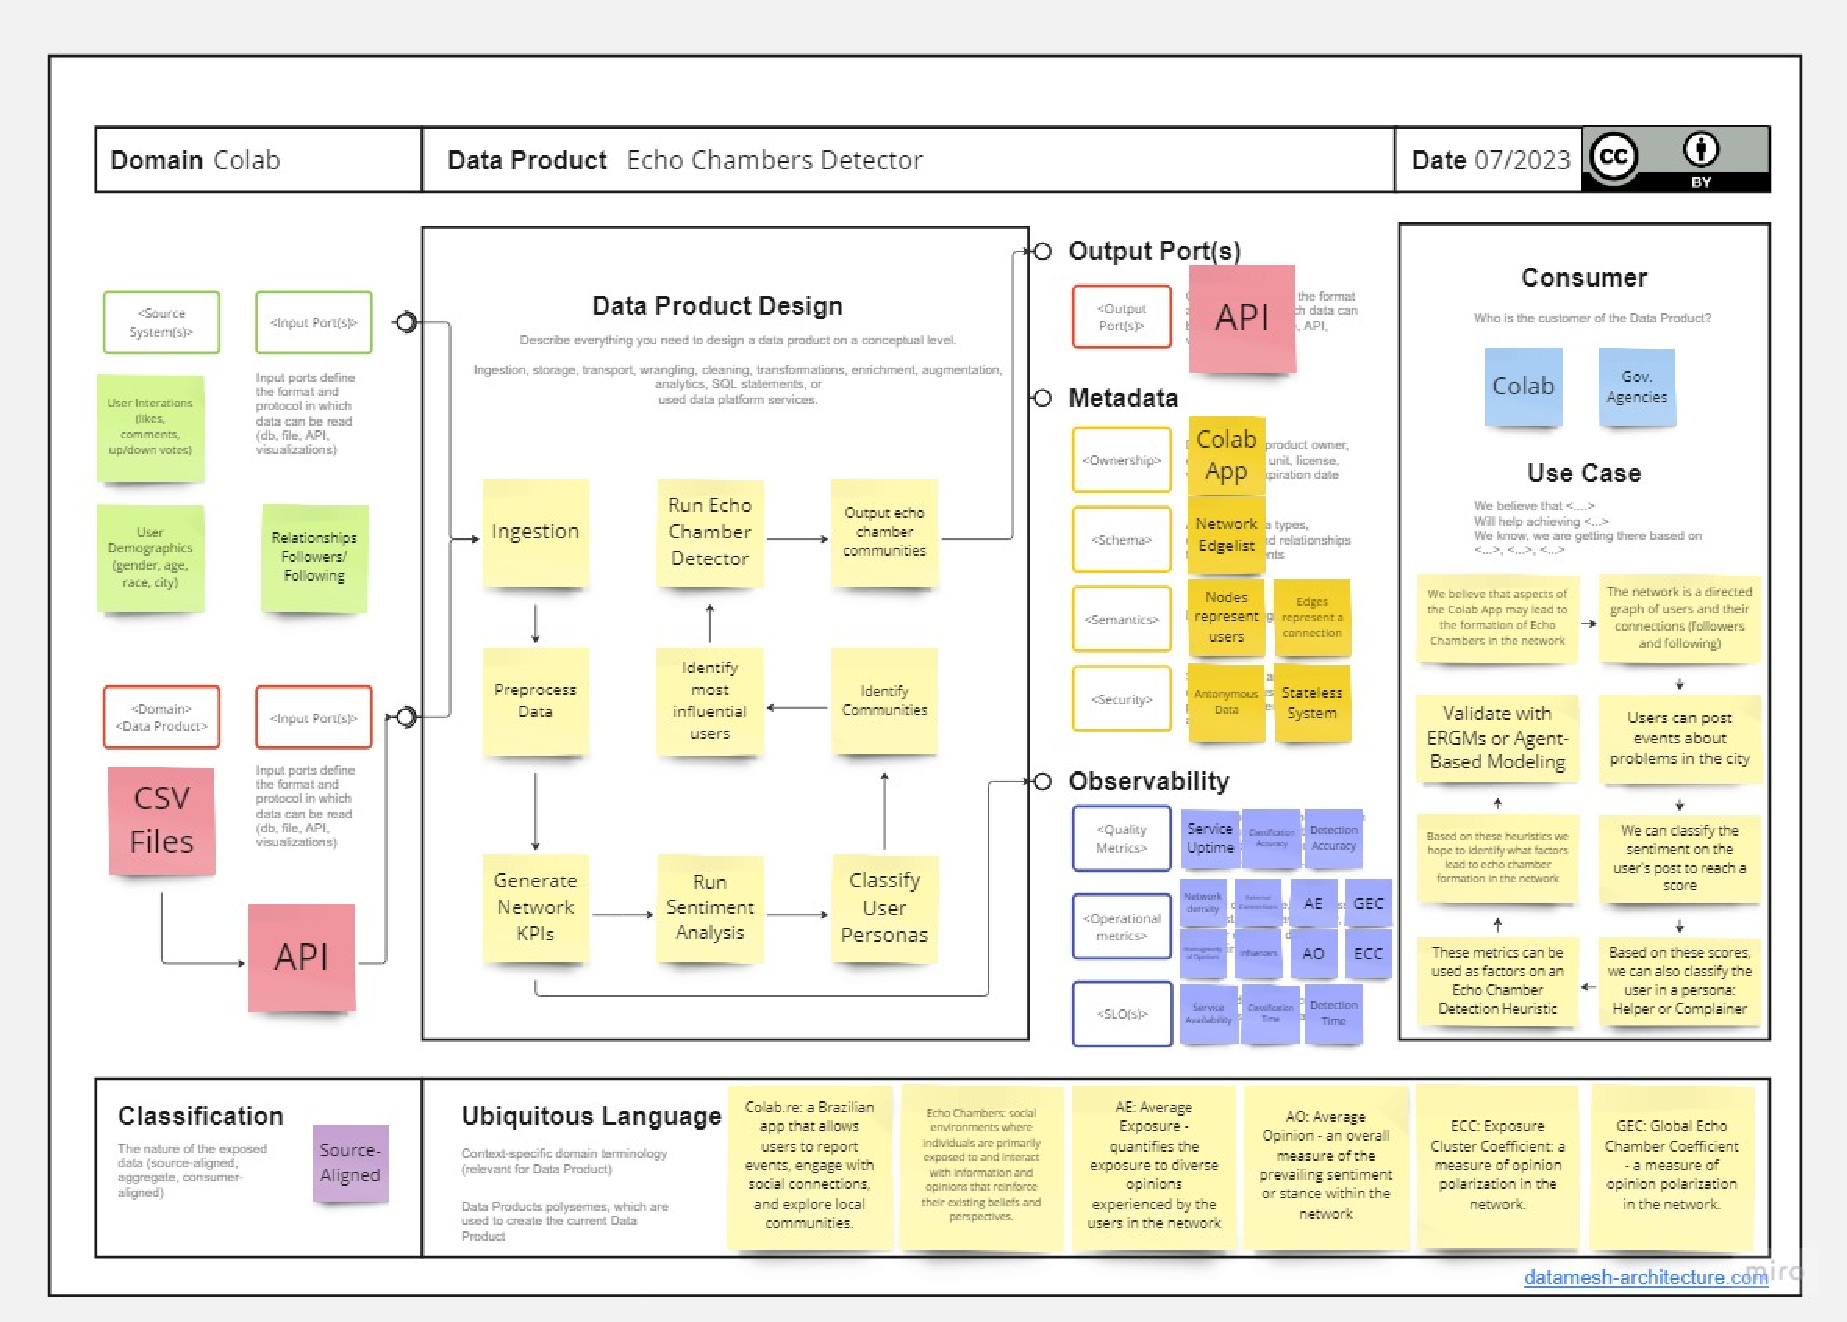
\includegraphics[scale=0.5]{tex/includes/data_canvas.pdf}
	\fautor
\end{figure}

Durante as discussões exploratórias com a equipe do Colab, elaboramos o Data Product Canvas como parte integrante da metodologia adotada para o desenvolvimento do aplicativo de detecção de câmaras de eco. O canvas proporcionou uma estrutura sólida e organizada para entendermos os requisitos do aplicativo e definirmos os diferentes elementos envolvidos em seu design e implementação.

Na seção de "Portos de Entrada", identificamos as interações dos usuários, como curtidas, comentários e votos positivos/negativos, juntamente com dados demográficos relevantes, como gênero, idade, raça e localidade. Além disso, consideramos as conexões entre usuários, representadas por seguidores e pessoas seguidas. Esses portos de entrada são fundamentais para a coleta dos dados necessários para análise e detecção de câmaras de eco na rede.

O design do produto de dados foi delineado em várias etapas, desde a ingestão dos dados até a geração de KPIs da rede, execução da análise de sentimentos, classificação das personas dos usuários, identificação de comunidades, detecção de usuários influentes, até a execução do detector de câmaras de eco e a saída das comunidades identificadas. Essa abordagem sequencial e bem definida permitirá uma análise abrangente e sistemática das câmaras de eco presentes na rede, fornecendo insights valiosos sobre sua formação e dinâmica.

Ao considerar os "Portos de Saída", optamos por utilizar uma API para disponibilizar as comunidades de câmaras de eco detectadas pelo aplicativo. Essa escolha nos permite fornecer acesso eficiente e acessível aos resultados obtidos, tanto para o próprio Colab App quanto para agências governamentais interessadas em entender e abordar a formação de câmaras de eco na rede.

A seção de "Metadados" do nosso canvas é particularmente relevante, pois aborda aspectos essenciais para a compreensão e governança adequada dos dados. Nesse contexto, especificamos que o aplicativo pertence ao Colab App e adotamos um esquema de dados baseado em uma lista de arestas da rede. A semântica do produto de dados é definida pelas entidades que representam os usuários e pelas conexões que representam as relações entre eles. Além disso, consideramos a segurança dos dados, garantindo que todas as informações coletadas sejam anônimas e que o sistema seja stateless.

A observabilidade é um aspecto crítico para garantir a qualidade e o desempenho do aplicativo. Nesse sentido, definimos métricas relevantes, como tempo de atividade do serviço, precisão da detecção, precisão da classificação, densidade da rede, conexões externas, homogeneidade de opiniões, influenciadores, opinião média, exposição média, coeficiente de agrupamento de exposição e coeficiente de câmaras de eco global. Essas métricas nos permitirão monitorar e avaliar o desempenho do aplicativo, bem como a eficácia da detecção de câmaras de eco na rede.

No contexto dos consumidores, identificamos o Colab App e agências governamentais como as partes interessadas em utilizar as comunidades de câmaras de eco detectadas. Esses consumidores poderão aproveitar os insights fornecidos pelo aplicativo para entender a formação das câmaras de eco e desenvolver estratégias eficazes para mitigar seus efeitos negativos.

Considerando o caso de uso do aplicativo, ressaltamos a crença de que certos aspectos do Colab App podem levar à formação de câmaras de eco na rede. Nesse contexto, o aplicativo foi projetado para permitir que os usuários postem eventos relacionados a problemas em suas cidades. Além disso, a análise de sentimentos é aplicada a essas postagens, fornecendo uma pontuação que permite classificar os usuários em personas. Essas métricas são fatores essenciais na heurística de detecção de câmaras de eco, que busca identificar quais fatores contribuem para a formação dessas câmaras. Por fim, planejamos validar nossos resultados utilizando modelos ERGMs (Exponential Random Graph Models) ou modelos baseados em agentes para confirmar a robustez das detecções feitas pelo aplicativo.

O uso do Data Product Canvas revelou-se essencial para estabelecer uma abordagem estruturada e colaborativa no desenvolvimento do aplicativo de detecção de câmaras de eco. Através desse framework, foi possível uma clara definição dos requisitos, elementos de design e aspectos operacionais do aplicativo, guiando todo o processo de desenvolvimento de forma sistemática.

Ao adotar o Data Product Canvas, buscamos não somente construir um aplicativo funcional, mas também obter uma compreensão aprofundada das dinâmicas de formação e impacto das câmaras de eco na rede do Colab App. Com uma definição clara dos portos de entrada, como as interações dos usuários e seus dados demográficos, e a utilização de técnicas de análise de sentimentos e classificação de personas, esperamos gerar insights valiosos para a mitigação dos efeitos negativos dessas câmaras.

Essa abordagem orientada pelo Data Product Canvas permite uma visão holística do aplicativo, contemplando desde a ingestão e pré-processamento dos dados até a identificação e classificação das comunidades de câmaras de eco. Com a identificação dos portos de saída, como uma API para disponibilizar as comunidades detectadas, buscamos assegurar a acessibilidade dos resultados tanto para os usuários do Colab App quanto para as agências governamentais interessadas.

Portanto, a aplicação do Data Product Canvas no desenvolvimento do aplicativo de detecção de câmaras de eco fortaleceu a estrutura do projeto, promovendo um processo colaborativo e possibilitando uma compreensão aprofundada das dinâmicas sociais envolvidas. Essa abordagem estruturada e integrada nos permite vislumbrar uma contribuição significativa para a identificação e mitigação das câmaras de eco no contexto do Colab App, fornecendo uma base sólida para a promoção de uma troca de informações mais diversificada e inclusiva na rede.

\section{Considerações Éticas e limitações}
Ao conduzir esta pesquisa, dedicamos especial atenção às considerações éticas e às questões de privacidade dos usuários. Todas as diretrizes éticas foram rigorosamente seguidas, e medidas foram adotadas para garantir a confidencialidade e o anonimato dos dados utilizados. Respeitamos a privacidade dos usuários do aplicativo Colab, tratando todas as informações de maneira sensível e em conformidade com as regulamentações e políticas de proteção de dados.

Obtivemos todas as autorizações necessárias para acessar e utilizar os dados relacionados aos usuários do aplicativo Colab, garantindo a legalidade e a conformidade com as diretrizes estabelecidas. Além disso, asseguramos que todas as informações sensíveis fossem tratadas com responsabilidade, adotando medidas de segurança adequadas para evitar qualquer divulgação não autorizada.

É importante ressaltar que todos os procedimentos adotados nesta pesquisa estão em conformidade com as diretrizes éticas estabelecidas pelo Comitê de Ética em Pesquisa de nossa instituição. O projeto foi submetido a uma análise minuciosa, considerando todos os aspectos éticos relacionados à coleta, análise e divulgação dos dados. A integridade e a validade dos resultados foram salvaguardadas por meio da adesão rigorosa às normas e regulamentos éticos.

Quanto às limitações do estudo, é válido destacar a natureza predominantemente quantitativa da pesquisa. Embora tenhamos empregado técnicas de análise de redes, algoritmos de agrupamento e detecção de comunidades, bem como a utilização de modelos epidemiológicos digitais, reconhecemos que uma abordagem exclusivamente quantitativa pode limitar a compreensão completa do fenômeno em estudo.

Para complementar a análise objetiva das interações dos usuários e a disseminação de informações nas câmaras de eco, é importante considerar abordagens qualitativas. Entrevistas e análise de conteúdo podem fornecer insights valiosos sobre as percepções, atitudes e motivações dos usuários envolvidos nas câmaras de eco. A combinação dessas abordagens quantitativas e qualitativas permitiria uma compreensão mais abrangente e rica do fenômeno.

É fundamental reconhecer e abordar as limitações inerentes a qualquer pesquisa, garantindo que os resultados sejam interpretados com cautela e considerando possíveis viéses ou lacunas no estudo. Ao fazê-lo, podemos avançar no conhecimento sobre as câmaras de eco no contexto do Colab App, contribuindo para uma compreensão mais completa desse fenômeno complexo e fornecendo subsídios para ações mitigadoras efetivas.

\section{Disponibilidade do Código-Fonte}
O código-fonte desenvolvido neste projeto está disponível em um repositório público no GitHub. Ele contém as implementações dos algoritmos de construção da rede social, algoritmos de agrupamento, modelos de epidemiologia digital e o desenvolvimento do painel em tempo real. O repositório pode ser acessado no seguinte endereço:\url{https://github.com/guinetik/colab-network-ec}.